\documentclass[11pt,a4paper]{article}

% Packages
%\usepackage{fullpage}
\usepackage[left=2cm,right=2cm,top=3.5cm,bottom=3.5cm]{geometry}
\usepackage{titling}
\usepackage{titlesec}
\usepackage{titletoc}
\usepackage[hidelinks]{hyperref}
\usepackage{float}
\usepackage{graphicx}
\usepackage{caption}
\usepackage{gensymb}
\usepackage{tabularx}	
\usepackage{listings}
\usepackage[usenames, dvipsnames]{color}
\usepackage{wallpaper}
\usepackage{setspace}
\usepackage{enumitem}
\usepackage{anyfontsize}
\usepackage{tikz}
\usepackage{nameref}
\usepackage[titles]{tocloft}
\usepackage{textcomp}
\usepackage{subcaption}
%\usepackage[obeyspaces]{url}

%Font settings
%\usepackage[T1]{fontenc}
\usepackage{lmodern} %For Standard
%\usepackage{helvet} %For Helvetica
\usepackage{classico} %For Classico
%\renewcommand{\familydefault}{\sfdefault}

% Document info
\title{Gramophone User Guide}
\author{Femtonics Ltd.}
\date{\today}

% Graphics foltder
\graphicspath{ {images/} }

% Python code formatting
\definecolor{dkgreen}{rgb}{0,0.6,0}
\definecolor{gray}{rgb}{0.5,0.5,0.5}
\definecolor{lightgray}{rgb}{0.9,0.9,0.9}
\definecolor{mauve}{rgb}{0.58,0,0.82}
\lstset{
  upquote=true,
  frame=tb,
  language=Python,
  aboveskip=3mm,
  belowskip=3mm,
  showstringspaces=false,
  columns=flexible,
  basicstyle={\small\ttfamily},
  numbers=left,
  numberstyle=\tiny\color{gray},
  keywordstyle=\color{blue},
  commentstyle=\color{dkgreen},
  stringstyle=\color{mauve},
  breaklines=true,
  breakatwhitespace=true,
  tabsize=3,
}




% Custom titlepage 
\addtolength{\wpYoffset}{-12.5cm}
\renewcommand{\maketitle}{
\begin{titlepage}
%\ThisULCornerWallPaper{1}{mouse.jpg}
\ThisLLCornerWallPaper{1}{arcualt_design_element.pdf}
\ThisCenterWallPaper{0.5}{femtonics-logo_silver_with_tagline.png}
\begin{center}

\classico{\scshape\Huge\thetitle}

\normalsize\thedate

\vspace{2.1cm}

%\includegraphics[scale=0.25]{Gramophone.jpg}
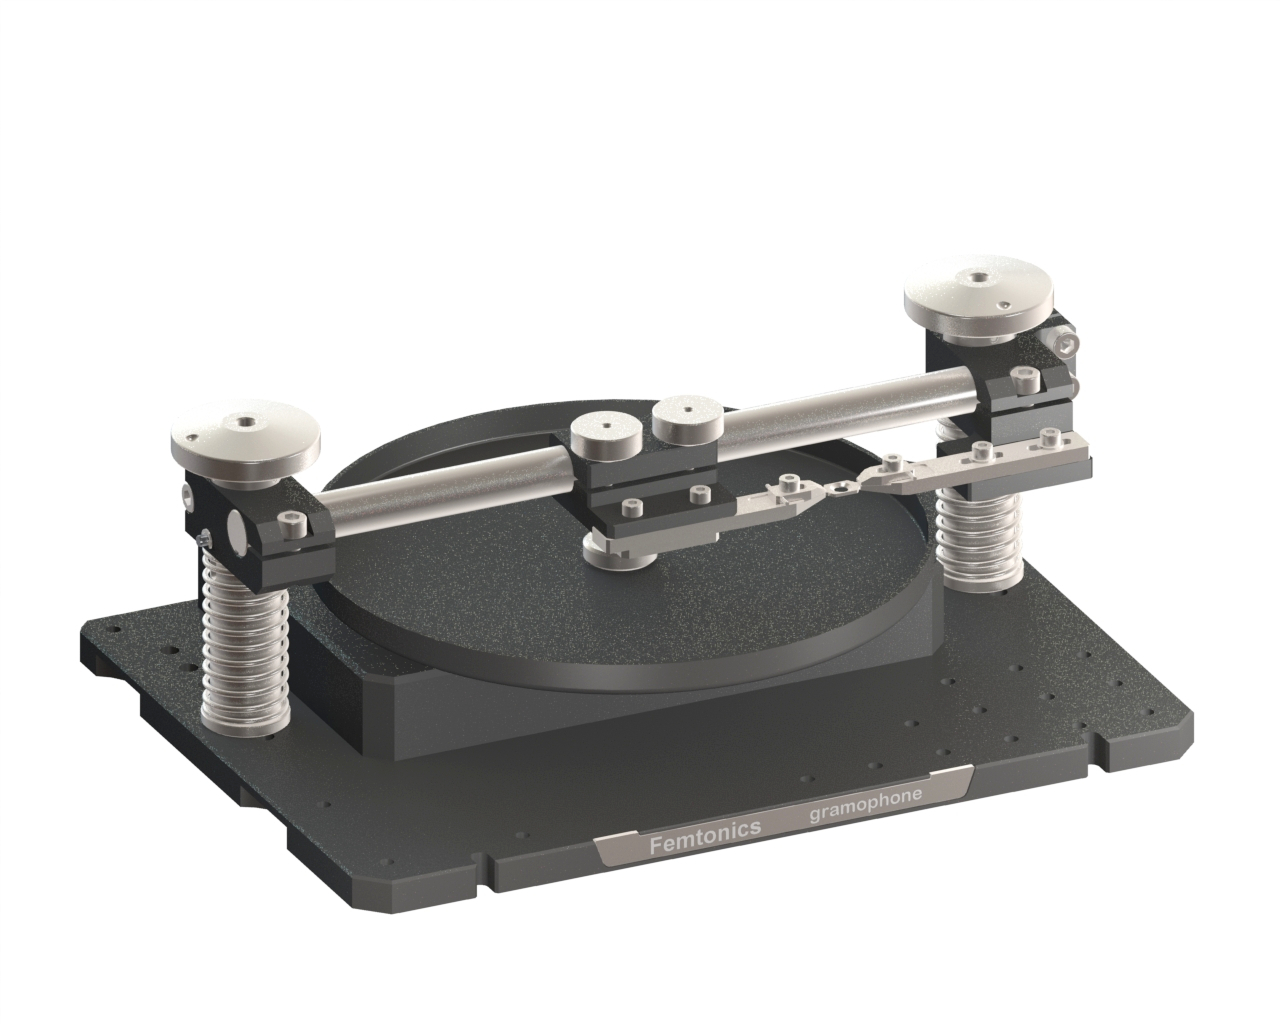
\includegraphics[width=.9\textwidth]{Gramophone_titlepage.JPG}



\end{center}
\end{titlepage}
}

% Levels under \section are not numbered
\setcounter{secnumdepth}{1} 

% TOC indentation and dotting
\setlength{\cftsecindent}{0em}
\setlength{\cftsubsecindent}{2em}
\setlength{\cftsubsubsecindent}{3em}
%\dottedcontents{section}[1.5em]{}{1.3em}{.6em}

% Custom section spacing and formatting
% -- Section
\titleformat{\section}
	{\Large\bf\raggedright} %\classico
	{\hspace{-1.5em}{\fontsize{50}{0}\selectfont\textcolor{lightgray}\thesection}} %\hspace{0em}
	{-0.5cm}
	{}
	[{\titlerule[1pt]}]
\titlespacing{\section}{0pt}{20pt}{7pt}

% -- Section*
\titleformat{name=\paragraph,numberless}
	{\Large\bf\raggedright}
	{\hspace{0em}}
	{-0.3cm}
	{}
	[{\titlerule[1pt]}]
\titlespacing*{\section}{0pt}{20pt}{7pt}

% -- Subsection
\titleformat{\subsection}
	{\large\bfseries}
	{\hspace{0cm}} %\hspace{-1cm}\textcolor{Gray}\thesubsection
	{0em}
	{}
	[]
\titlespacing{\subsection}{0pt}{15pt}{3pt}

% -- Subsubsection
\titleformat{\subsubsection}
{\bfseries}
{\hspace{0cm}}
{0em}
{}
[]
\titlespacing{\subsubsection}{0pt}{15pt}{3pt}

%\let\mtcontentsname\contentsname
%\renewcommand\contentsname{\MakeUppercase\mtcontentsname}
%\renewcommand\cftaftertoctitle{\par\noindent\hrulefill\par\vskip-4.3em}

% Don't indent paragraphs
\setlength{\parindent}{0in}

% Custom list for parameters
\newlist{paramlist}{itemize}{1}
\setlist[paramlist]{label=$\triangleright$}
\newcommand{\param}[1]{\item \texttt{#1} -}

% Command for making editorial notes
\newcommand{\enote}[1]{\textcolor{RubineRed}{#1}}

\newcommand{\note}[1]{\textit{Note: {#1}}}

\newcommand{\hlink}[1]{\href{#1}{#1}}
\newcommand{\mlink}[1]{\href{mailto:#1}{#1}}

% ------------------------ BODY ------------------------
\begin{document}
\maketitle
%\ULCornerWallPaper{1}{2016_header.jpg}
\ULCornerWallPaper{1}{Femtonics_header_letter.png}
%\LLCornerWallPaper{1}{2016_footer_info.jpg
\LLCornerWallPaper{1}{Femtonics_footer_letter.png}
\tableofcontents

\newpage
\section{Introduction}
The Gramophone system is a single dimension locomotion tracking device for head-restrained mice that has two modes of operation. It can either be used for high-accuracy velocity recording in conjunction with a two-photon microscope, or as a control interface for behavioural training in a virtual linear maze.


\section{Compatibility}
The system is compatible with Microsoft Windows 7 or newer. To run the computer software, a Python 3.6 interpreter is required.

The system can be used in conjunction with Femtonics SMART microscopes and certain custom built models. To get further information about compatibility with your device, please contact Femtonics Ltd. at \mlink{info@femtonics.eu}.

\section{Links}
\begin{itemize}
\item Python Package Index - \hlink{https://pypi.org/project/GramophoneTools}
\item GitHub - \hlink{https://github.com/Femtonics/GramophoneTools}
\item Documentation - \hlink{http://gramophone.femtonics.eu/}
\item User guide - \hlink{http://gramophone.femtonics.eu/user\_guide.html}
\end{itemize}

%\section{Warranty}
%\enote{TODO}

\section{Contact}
If you need further assistance, please contact Femtonics Ltd. via e-mail at \mlink{info@femtonics.eu} or visit our website \hlink{http://femtonics.eu/contact}

\section{Cleaning instructions}
\subsection{Disk}
Remove the disk (Figure \ref{fig:gram_overview}a) by unscrewing its mounting screw (Figure \ref{fig:gram_overview}b) and clean it with warm soapy water. The disk can be sterilized with alcohol-based disinfectants.
% and is resistant to temperatures up to \enote{add temp resisitance when available} \degree C.

\subsection{System}
Disconnect the device from the computer by unplugging the USB cable (Figure \ref{fig:gram_ports}b). Clean the device with a damp cloth.

\newpage
\section{Hardware overview}
\begin{figure}[h] %<left> <lower> <right> <upper>
\centering
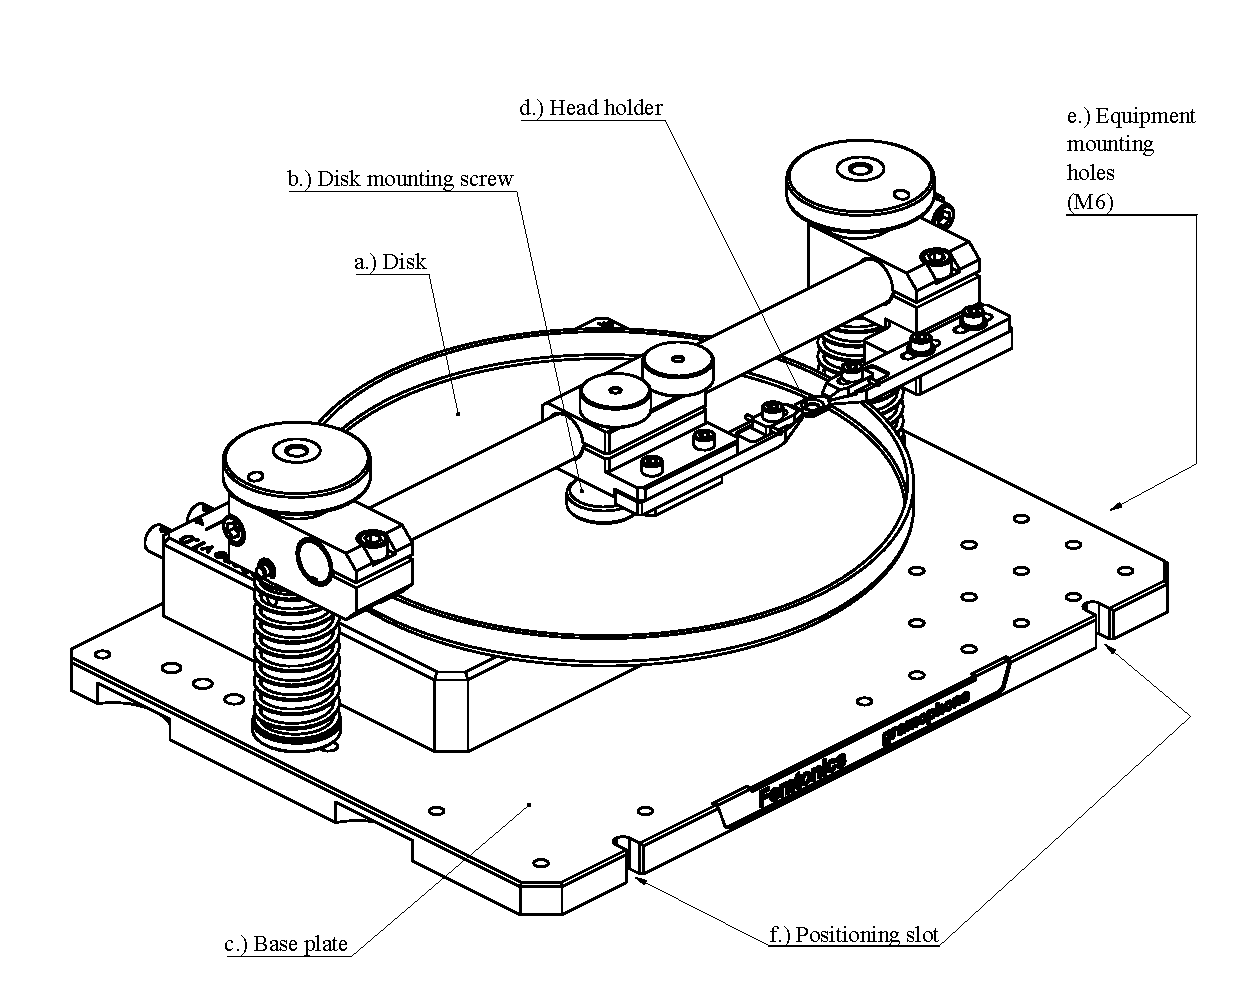
\includegraphics[clip, trim=1cm 0cm 0cm 1cm, width=1.00\textwidth]{labels_overview.PDF}
\caption{Overview of the Gramophone device.}
\label{fig:gram_overview}
\end{figure}


\subsection{Specifications}
\begin{itemize}
\item Operating temperature: 0-60 \degree C
\item Relative humidity during operation:  $<$ 90\%, avoid condensation 
\item Power requirements - 5V DC @500mA via USB. The use of passive USB hubs is prohibited.
\end{itemize}

\subsection{Inputs and Outputs}
\begin{figure}[H] %<left> <lower> <right> <upper>
\centering
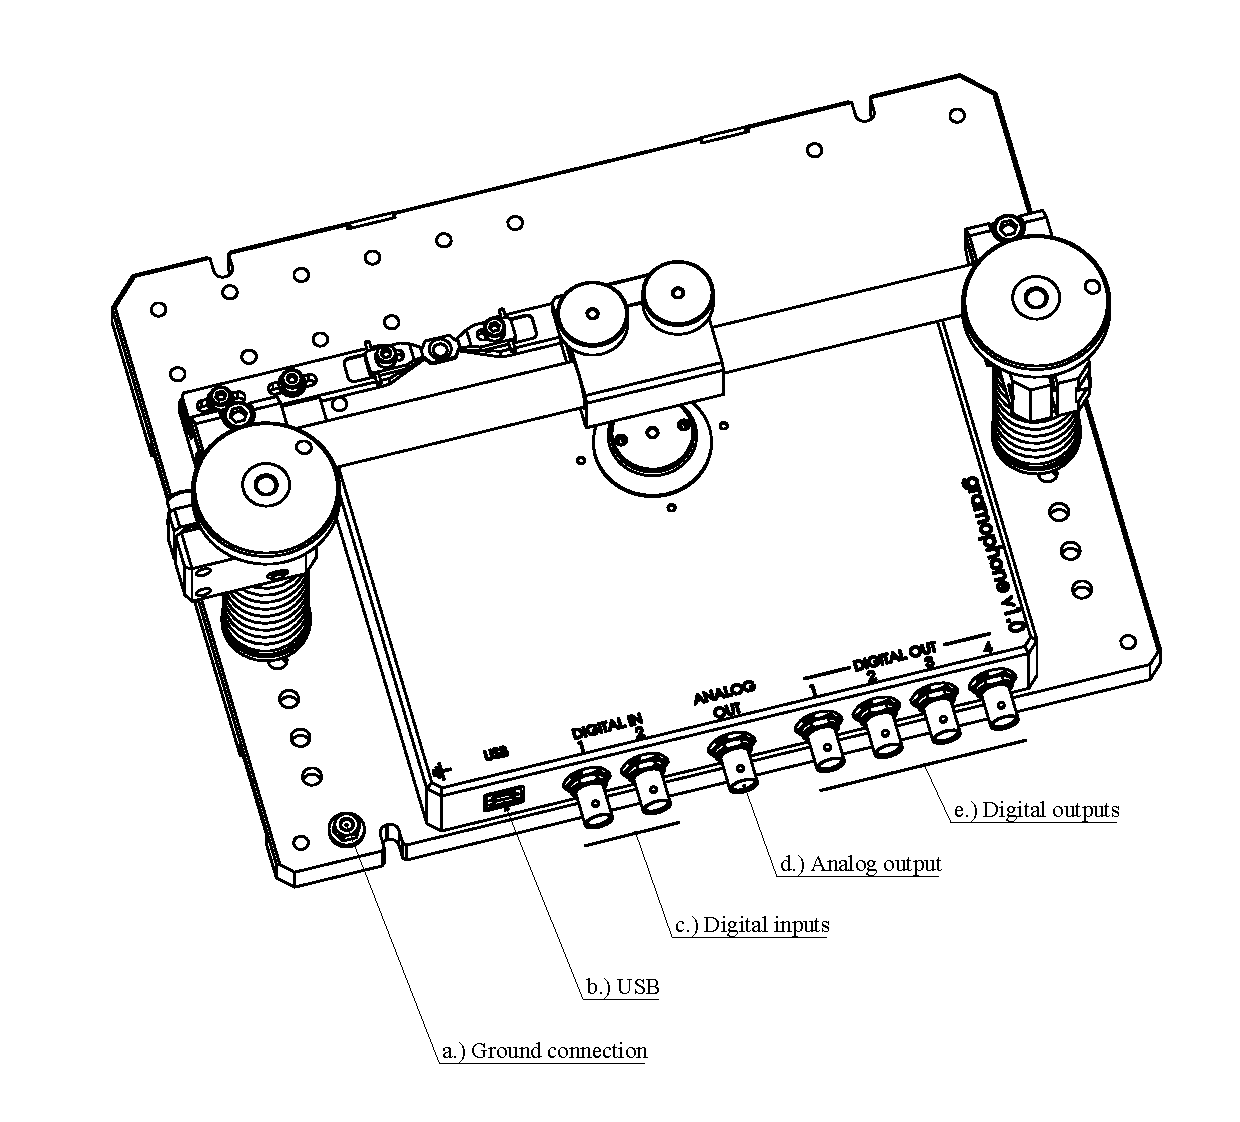
\includegraphics[clip, trim=1cm 1cm 0cm 1cm, width=1.00\textwidth]{labels_ports.PDF};
\caption{Inputs and outputs on the Gramophone device.}
\label{fig:gram_ports}
\end{figure}

The Gramophone connects to the computer via USB 2.0. A cable is provided with the system.

The system has 7 full-sized BNC connectors:
\begin{itemize}
\item 4 digital outputs (Figure \ref{fig:gram_ports}e) that are connected to ground if their state is set to low, and connected to +5 volts if their state is set to high.

high: 4 - 5,5V @ 3mA

low:  0 - 1V   @ -3mA

\item 2 digital inputs  (Figure \ref{fig:gram_ports}c) that are considered to be in a low state if the voltage on them is below 1 volts and high if the voltage is above 4 volts. 

high: 4-6V @3mA

low:  0 - 1V


\item 1 analogue differential output (Figure \ref{fig:gram_ports}d) that is proportional to the current velocity of the animal.

V\textsubscript{common mode}:  0V

V\textsubscript{differential}: 0 - 2,5V
\end{itemize}
All digital IOs are galvanically isolated from the control circuit.

\subsection{Ground connection}
The system has a single banana plug connection (Figure \ref{fig:gram_ports}a) on the base plate marked with a ground sign. Always connect this to a ground with the included cable before using the device.

\subsection{Height adjustment \label{sec:height_adjust}}
The distance between the head-holder and the disk can be adjusted to fit mice of any size comfortably.
\begin{enumerate}
\item Loosen the locking screws with the included hex key (Figure \ref{fig:gram_height_1}a and b).
\item Adjust both height-adjustment knobs (Figure \ref{fig:gram_height_1}d) at the same time until the desired height is reached. Turning the knobs clockwise raises the head-holder relative to the disk, while turning it counter-clockwise lowers it (Figure \ref{fig:gram_height_2}). You can use the height reference notches Figure \ref{fig:gram_height_1}e) to make sure that the head holder is not tilted.
\item Lock the position by tightening the locking screws with the included hex key (Figure \ref{fig:gram_height_1}a and b).
\end{enumerate}

\begin{figure}[H] %<left> <lower> <right> <upper>
\centering
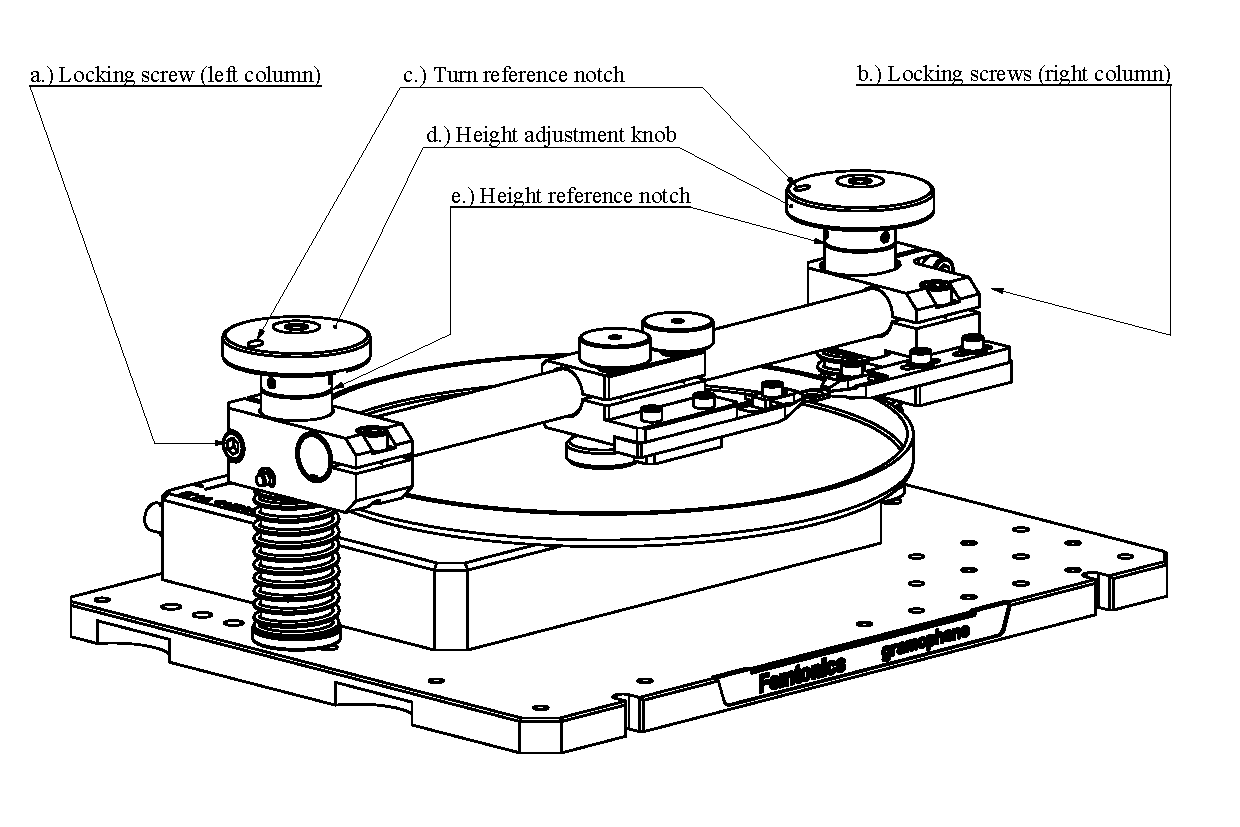
\includegraphics[clip, trim=0cm 0cm 0cm 1cm, width=1.00\textwidth]{labels_height_1.PDF};
\caption{Inputs and outputs on the Gramophone device.}
\label{fig:gram_height_1}
\end{figure}

\begin{figure}[H] %<left> <lower> <right> <upper>
\centering
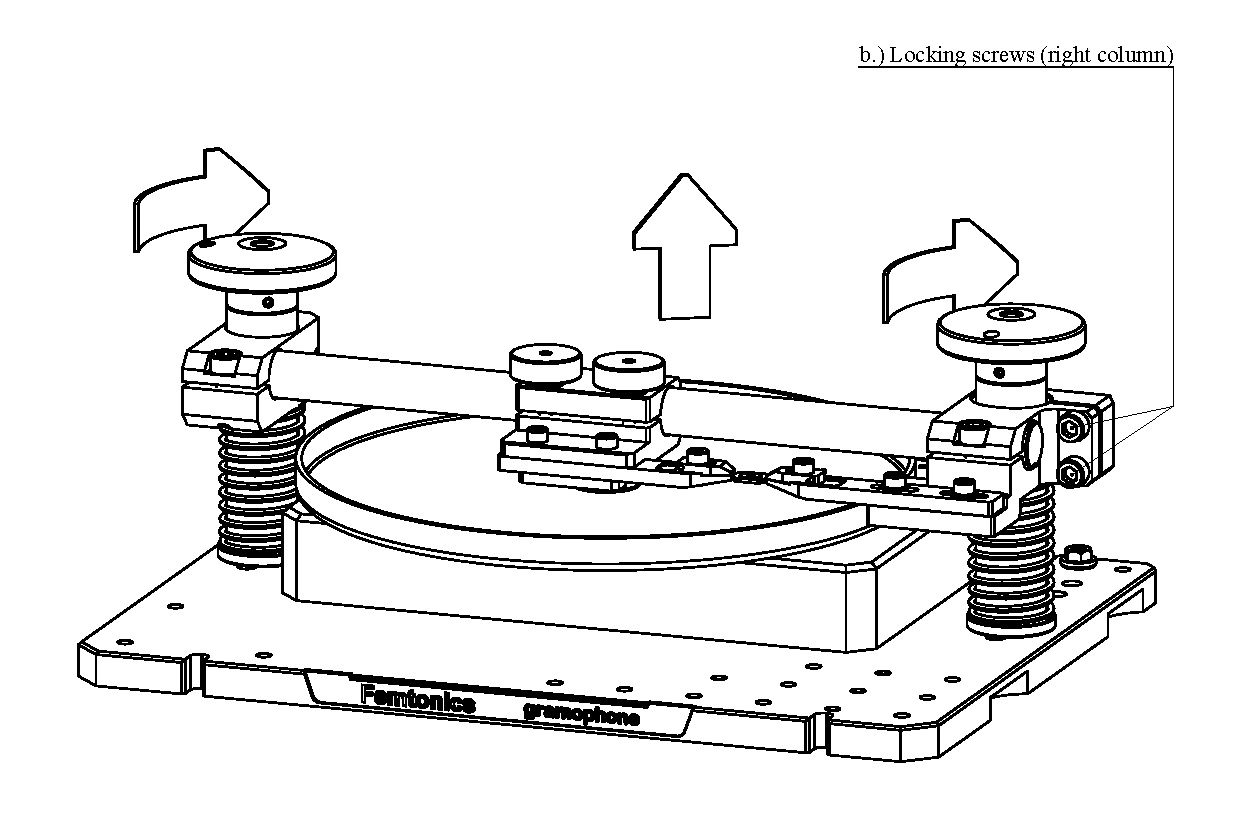
\includegraphics[clip, trim=1cm 1cm 0cm 0cm, width=1.00\textwidth]{labels_height_2.PDF};
\caption{Inputs and outputs on the Gramophone device.}
\label{fig:gram_height_2}
\end{figure}



\subsection{Position adjustment}
The position of the head-holder can be adjusted both sideways and back and forth to position the mouse anywhere on the disk.

\subsubsection{Sideways adjustment}
\begin{enumerate}
\item Loosen the two locking screws on the cylindrical axle with the knobs (Figure \ref{fig:labels_side}a).
\item Move the left part of the head-holder to the desired position by sliding the whole assembly on the axle.
\item Lock the left part of the head-holder with the knobs in the desired position (Figure \ref{fig:labels_side}a).
\item Loosen the two screws (Figure \ref{fig:labels_side}b) on the right part of the head-holder.
\item Adjust the right part until the head-holder fits a head-mount perfectly. \note{It is best practice to keep a head-mount handy for this.}
\item Lock the right part in place with the two locking screws (Figure \ref{fig:labels_side}b).
\end{enumerate}

\begin{figure}[H] %<left> <lower> <right> <upper>
\centering
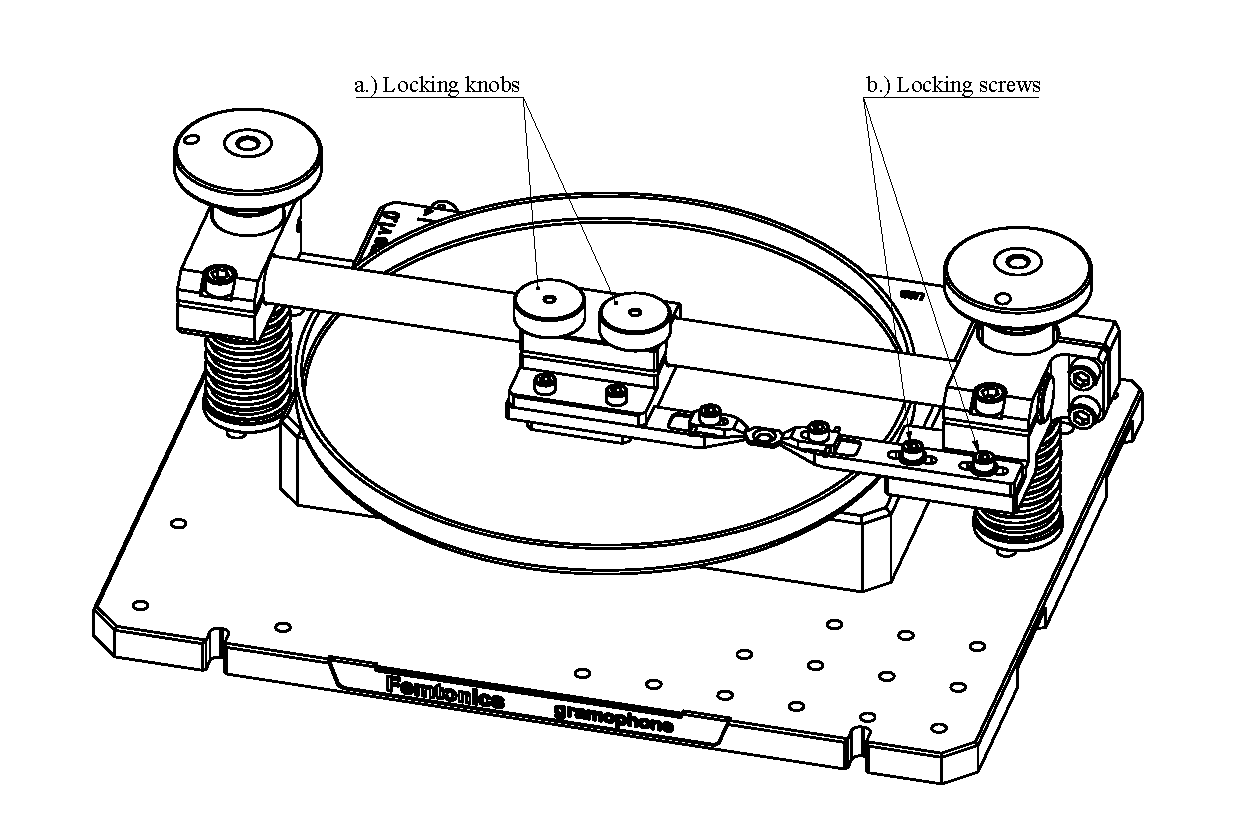
\includegraphics[clip, trim=1cm 0cm 1cm 1cm, width=1.00\textwidth]{labels_side.PDF};
\caption{Sideways adjustment of the mouse on the Gramophone.}
\label{fig:labels_side}
\end{figure}

\subsubsection{Back-and-forth adjustment}
\begin{enumerate}
\item Make sure that the height-adjustment screws are tightened (Figure \ref{fig:gram_height_1}a and b).
\item Remove the screws holding the columns in place (Figure \ref{fig:gram_back}a) with the included hex key.
\item Position the columns in the desired location such that their centres line up with a pair of mounting holes on the base plate.
\item Put back the removed screws in the new location and tighten them with the included hex key (Figure \ref{fig:gram_back}a).
\end{enumerate}

\begin{figure}[H] %<left> <lower> <right> <upper>
\centering
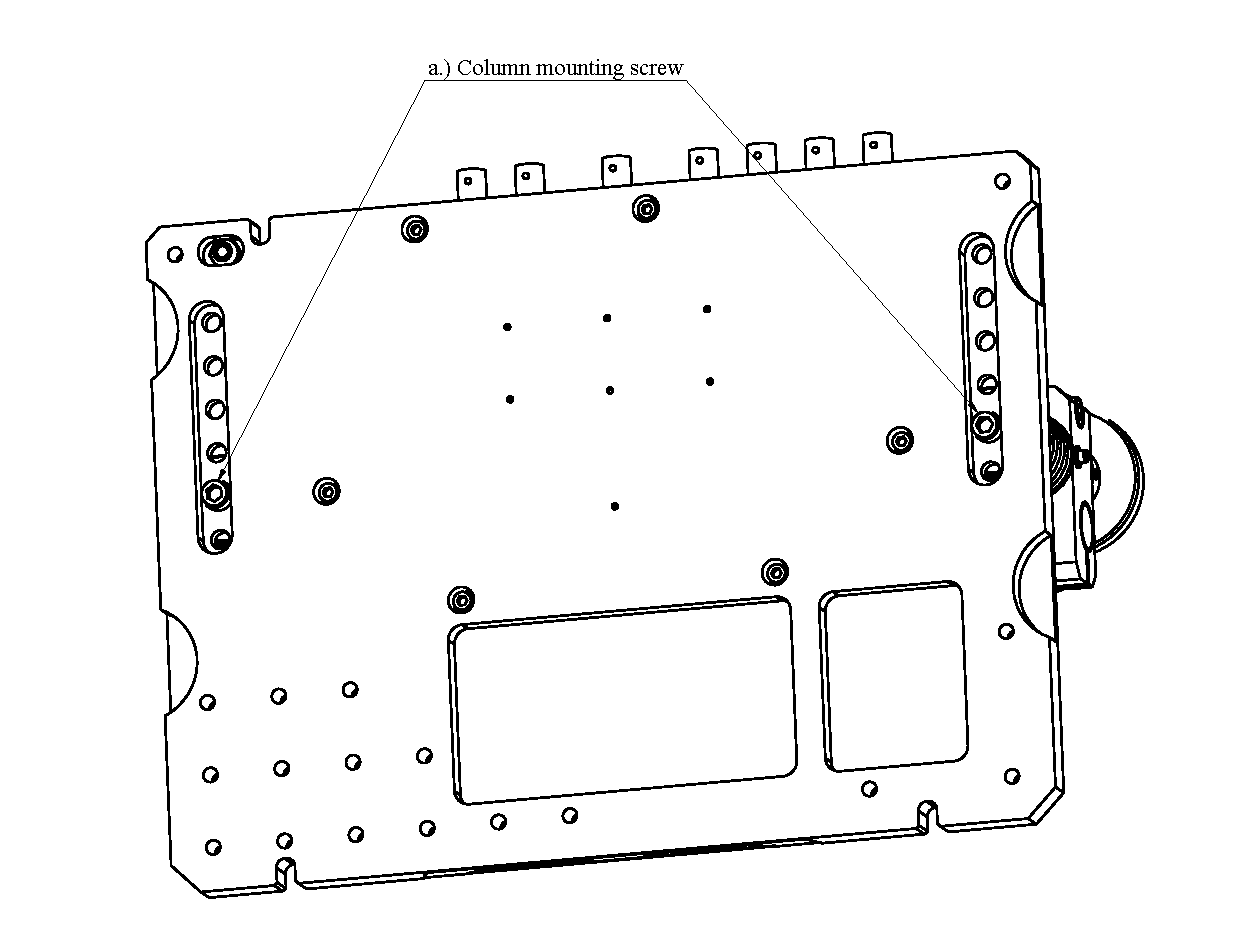
\includegraphics[clip, trim=1cm 0cm 0cm 0cm, width=1.00\textwidth]{labels_back.PDF};
\caption{Inputs and outputs on the Gramophone device.}
\label{fig:gram_back}
\end{figure}

\newpage
\section{Software installation}
\subsection{Drivers}
No additional drivers are required for the Gramophone system. It operates as a HID (Human Interface Device), for which, all drivers are provided by modern operating systems.

\subsection{Python interpreter \label{sec:python_install}}
To run the computer software of the Gramophone system, a Python 3.6 interpreter has to be installed. To install it, download the latest Miniconda installer for your version of Windows
(links: 
\href{https://repo.continuum.io/miniconda/Miniconda3-latest-Windows-x86.exe}{\textbf{32-bit}}
or
\href{https://repo.continuum.io/miniconda/Miniconda3-latest-Windows-x86_64.exe}{\textbf{64-bit}}) from the \href{https://conda.io/miniconda.html}{\textbf{Conda website}}.
\\

\note{If you are not sure which version of Windows you are using, you can check by pressing the Win+Pause/Break key combination to open the System window and check under System $\rightarrow$ System type, or by right-clicking the Start menu, choosing System and checking under Device specifications $\rightarrow$ System type.}\\


Follow the installation steps:
\begin{enumerate}

\item Start the downloaded .exe file (Figure~\ref{fig:miniconda_install_1}). Click Next.
	\begin{figure}[H]
	\centering
	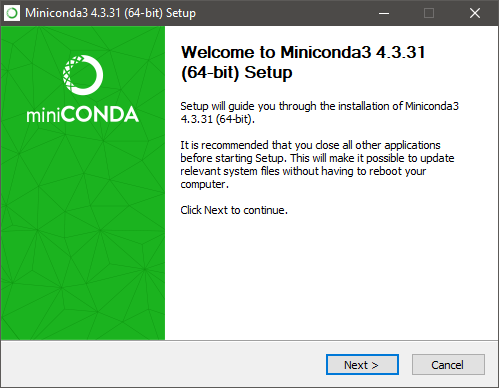
\includegraphics[scale=0.8]{miniconda_install_1.PNG}
	\caption{The Miniconda installer's welcome screen.}
	\label{fig:miniconda_install_1}
	\end{figure}
	
\newpage	
\item Agree to the License Agreement (Figure~\ref{fig:miniconda_install_license}).
	\begin{figure}[H]
	\centering
	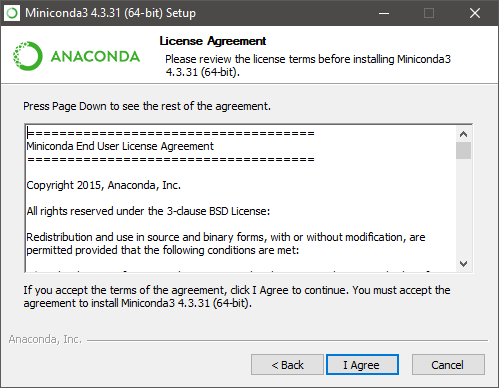
\includegraphics[scale=0.8]{miniconda_install_license.PNG}
	\caption{Agree to the License Agreement.}
	\label{fig:miniconda_install_license}
	\end{figure}


\item If multiple users will be using the same machine, install for all users (Figure~\ref{fig:miniconda_install_users}). Click Next.
	\begin{figure}[H]
	\centering
	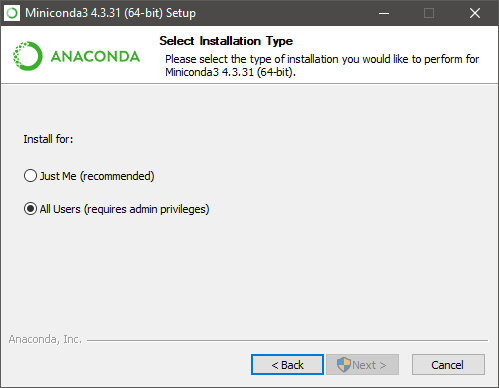
\includegraphics[scale=0.8]{miniconda_install_users.PNG}
	\caption{Install for all users if you use multiple users on the computer.}
	\label{fig:miniconda_install_users}
	\end{figure}

\newpage
\item Leave the installation directory as the default (Figure~\ref{fig:miniconda_install_dir}). Click Next.
	\begin{figure}[H]
	\centering
	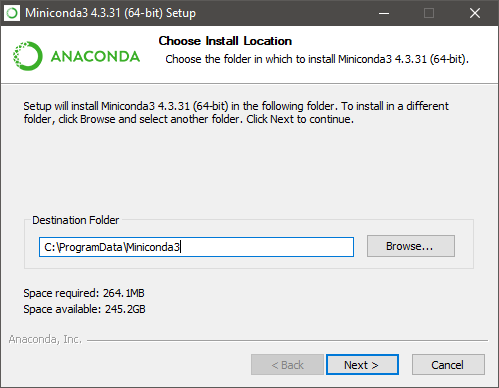
\includegraphics[scale=0.8]{miniconda_install_dir.PNG}
	\caption{Leave the install directory as the default if possible.}
	\label{fig:miniconda_install_dir}
	\end{figure}


\item Add Anaconda to the system PATH variable and register it as the system's Python 3.2 interpreter (Figure~\ref{fig:miniconda_install_options}). Click Install. 

\note{If you already have other versions of Python installed, leave these options unchecked and make sure you execute all Gramophone software from the Anaconda Prompt.}

	\begin{figure}[H]
	\centering
	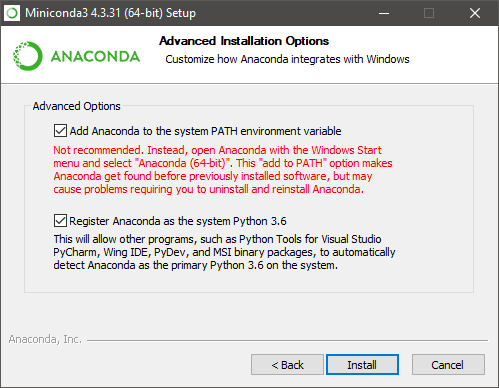
\includegraphics[scale=0.8]{miniconda_install_options.PNG}
	\caption{Check both options.}
	\label{fig:miniconda_install_options}
	\end{figure}

\newpage
\item Wait for the installation to finish (Figure~\ref{fig:miniconda_install_done}). Click Next.
	\begin{figure}[H]
	\centering
	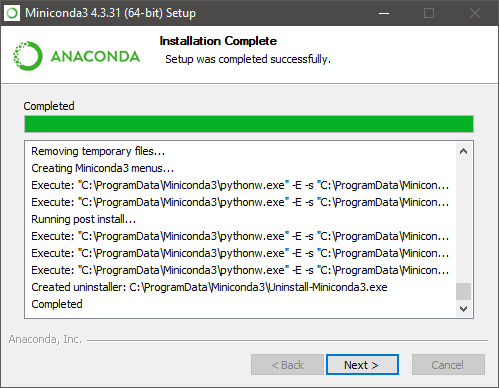
\includegraphics[scale=0.8]{miniconda_install_done.PNG}
	\caption{Wait for installation to finish.}
	\label{fig:miniconda_install_done}
	\end{figure}


\item Exit the installer by clicking Finish (Figure~\ref{fig:miniconda_install_done2}).
	\begin{figure}[H]
	\centering
	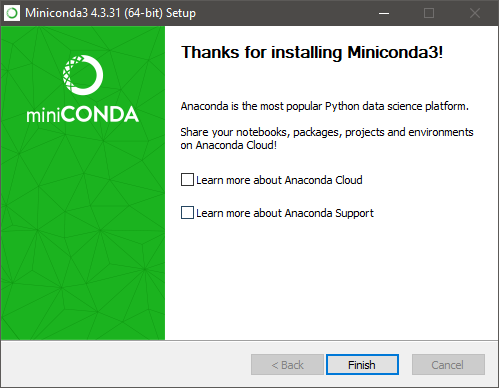
\includegraphics[scale=0.8]{miniconda_install_done2.PNG}
	\caption{Exit the installer.}
	\label{fig:miniconda_install_done2}
	\end{figure}

\end{enumerate}

\newpage
\subsection{Python modules}
All Gramophone related modules are collected in a single python package. To install it run the following command \textbf{as an administrator} in Windows Power Shell, Command Prompt or Anaconda Prompt:
\begin{verbatim}
pip install GramophoneTools
\end{verbatim}

\note{In Windows 10 you can open an Power Shell window as an administrator by right clicking on the start menu and choosing the "Windows PowerShell (Admin)" option.}

\subsubsection{Updating}
To find out if there is a newer version available run:
\begin{verbatim}
pip list -o
\end{verbatim}

If GramohoneTools shows up in the list you can update it by running:
\begin{verbatim}
pip install -U GramophoneTools
\end{verbatim}

\subsection{Associating .py files with the Python interpreter}
To start Python scripts (files with .py extension) with a double click in Windows you have to associate them with the Python interpreter (python.exe). To do so right click on any file with a .py extension under the "Open with" menu select the "Choose an other app" option. In the popup window choose the "Look for an other app on this PC" (you might need to open the "More apps" section). In the browser window that opened navigate to the location of python.exe. If you installed Miniconda with the default location this should be: \path{C:\ProgramData\Miniconda3\python.exe}

\note{The ProgramData folder is hidden in Windows so you have to type the location in the address bar to navigate there, or make hidden files and folders visible.}

\subsection{Associating .vlg files with the GramophoneTools Recorder}
The velocity recorder produces .vlg files as an output (see: \ref{sec:recorder_out}). To open these in the Recorder, right click on a .vlg file, select open with, search for an application on the computer and select \texttt{gramrec.exe} in the scripts folder of your Python installation. If you installed Python as described above (see: section \ref{sec:python_install}) this can be found here: \path{C:\ProgramData\Miniconda3\Scripts}.

\note{The ProgramData folder is hidden in Windows so you have to type the location in the address bar to navigate there, or make hidden files and folders visible.}

\note{You can also make a shortcut for \texttt{gramrec.exe} on the desktop to make starting it easier.}

\section{Software overview}
The GramophoneTools package has three modules. The \texttt{Comms} module handles all communication with the device. This can be used to develop your own application for the Gramophone. The Recorder module is an application with a GUI (Graphical User Interface) that can be used to record the animals velocity in a triggered manner. The LinMaze module is a collection of tools used to generate a 2 dimensional linear maze the mouse can navigate. Events and Rules can be added to this maze to implement various conditioning tasks.

After installing the GramophoneTools package, you can use a number of commands. The \texttt{gramrec} command simply starts the Recorder application. You can include a path to a .vlg file as a command line argument to open it with the recorder. The \texttt{gram} command can be used for various things, run \texttt{gram help} to find out more.

\note{You can open a terminal for these commands in Windows 10 by right clicking the start menu and selecting the 'Windows PowerShell' option, or you can run them in the Run window by pressing 'Win+R'.}

\note{You can create shortcuts for these commands by right clicking where you want the shortcut to be (eg. on the Desktop) and entering the command as the location of the item.}

\section{Recorder module} 
The Gramophone recorder is software that can make high accuracy velocity recordings. To keep the velocity records in sync with two-photon measurements the digital input 1 (Figure \ref{fig:gram_ports}c) is used as a trigger input for recordings. 

	\begin{figure}[H]
	\centering
	\begin{tikzpicture}[x=1cm,y=1cm]
	\node[anchor=south west] at (0,0) {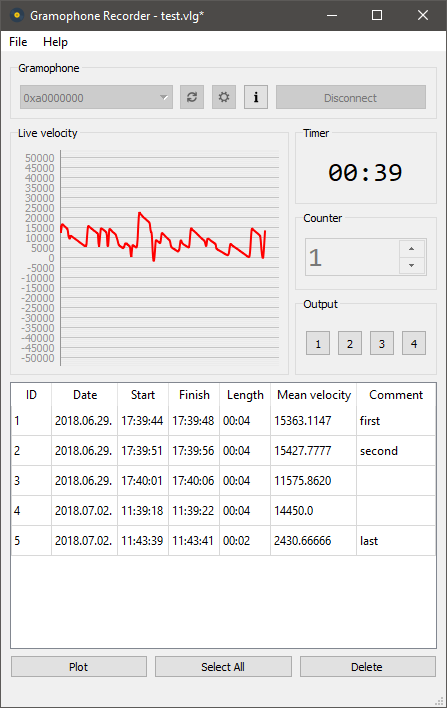
\includegraphics[scale=0.49]{pyGram_recording.PNG}};
	%\draw[gray,very thin] (0,0) grid (6,10);
\draw[<-] (5.5,8) --++ (3,1) --++ (3,0) node[above=3pt,anchor=south east,inner sep=0]{Connect button};
\draw[<-] (5.5,7.0) --++ (3,1) --++ (3,0) node[above=3pt,anchor=south east,inner sep=0]{Internal timer};
\draw[<-] (5.5,6.0) --++ (3,1) --++ (3,0) node[above=3pt,anchor=south east,inner sep=0]{Record counter};\draw[<-] (5.5,5.0) --++ (3,1) --++ (3,0) node[above=3pt,anchor=south east,inner sep=0]{Output control};

%\draw[<-] (2.5,9) --++ (-3,3) --++ (-5,0) node[above=3pt,anchor=south west,inner sep=0]{Refresh, settings and info button};
\draw[<-] (0.5,8) --++ (-3,1) --++ (-3,0) node[above=3pt,anchor=south west,inner sep=0]{Gramophone list};
\draw[<-] (0.5,6) --++ (-3,1) --++ (-3,0) node[above=3pt,anchor=south west,inner sep=0]{Live velocity graph};
\draw[<-] (0.5,2.5) --++ (-3,1) --++ (-3,0) node[above=3pt,anchor=south west,inner sep=0]{List of records};
\draw[<-] (0.5,0.7) --++ (-3,1) --++ (-3,0) node[above=3pt,anchor=south west,inner sep=0]{Record tools};
\end{tikzpicture}
	\caption{The user interface of the Gramophone recorder during recording.}
	\label{fig:pygram_recording}
	\end{figure}

\subsection{Useage}
To accurately record velocity with the Gramophone system follow these steps.

\subsubsection{Hardware setup}
\begin{enumerate}
\item Fix the mouse in the head holder. If necessary, adjust the height of the holder as explained in the  \nameref{sec:height_adjust} section.
\item Put the Gramophone with the mouse into the microscope, such that the craniotomy window on the head of the mouse lines up with the microscope's objective perfectly.
\item Connect the grounding point to a ground with the included cable (Figure \ref{fig:gram_ports}a).
\item Connect the digital output of the microscope with a digital input of the Gramophone (Figure \ref{fig:gram_ports}c) with a BNC cable.
\item Connect the Gramophone to the computer with the included USB cable (Figure \ref{fig:gram_ports}b).
\end{enumerate}

\subsubsection{Microscope configuration}
Configure the microscope to pull its digital output to hight for the time period you wish to record (eg.: pull to high when the shutter opens and to low when it closes).

\subsubsection{Software setup}
\begin{enumerate}
\item Start the Gramophone recorder with the icon on the Desktop or from the terminal with the \texttt{gramrec} command.
\item Select the Gramophone you wish to record from the dropdown list (see: Figure \ref{fig:pygram_recording}). If you can't find the connected device in the list, you can refresh it with the button next to it.
\item Click the gear button next to the list of Gramophones and in the window that opened set the trigger channel to the input you connected the microscope to.
\item Click the Connect button (see: Figure \ref{fig:pygram_recording}). The current velocity will be plotted on the Live velocity plot.
\item Start your measurement protocol in MES or MESc, the recorder will automatically capture velocity for every measurement unit.
\item You can see the velocity records on the List of records (Figure \ref{fig:pygram_recording}). You can select any number of records with the mouse and plot or delete them with the Record tools below the list.

\end{enumerate}

\subsection{Recording results \label{sec:recorder_out}}
The velocity log file is an HDF5 file with a \texttt{.vlg} extension. For more information about it's structure please visit the \href{http://gramophone.femtonics.eu/gramrec_out.html}{\textbf{online documentation of the Recorder module}}.

\section{LinMaze module}
LinMaze is a simple virtual linear maze system. It can generate patterns based on parameters and stitch these patterns together into an endless loop the mouse can navigate in using the Gramophone. Optionally, you can define rules to condition the mouse to a task eg. to differentiate between different patterns and behave accordingly.

\subsection{Levels}
To use the software you have to make a Python script that defines your Level. A Level is a collection of patterns, events and rules.
\\
To make a new Level you have to make a small Pyton script. All levels should start by importing the Level object and an \lstinline{if} statement that is needed for multithreading to work properly. After the \lstinline{if} statement you can start constructing your Level. Be sure to put 4 spaces in front of every line from now on.

\note{You can comment out lines by adding a \texttt{\#} character in front or make multiple line comment by wrapping with triple \texttt{\textquotesingle} characters \lstinline{''' like this '''}. Comments will be coloured green in the following examples.}
\\

First create a Level object. In these examples I will call mine \texttt{LVL}.

\begin{lstlisting}
''' An example level for LinMaze '''
from GramophoneTools.LinMaze.Level import Level
if __name__ == '__main__':
	LVL = Level(
		name = 'myFirstLevel',
		screen_res = (1280, 1024),
		zone_offset = 720,
		transition_width = 100,
		rgb = (0,0,1)
		)
\end{lstlisting}

The parameters for the Level are:
\begin{paramlist}  
\param{name} can be any string, this will show up in default file names.
\param{screen\_res} two integer numbers in parentheses, separated by commas. These give the resolution of the screen that the level will be running on.
\param{zone\_offset} an integer number that gives where the borders of the zones should be on the screen. Eg. If you set it to half the horizontal resolution, zones will be entered when they reach the middle of the screen from the right and are left when the last pixel of the frame leaves the middle.
\param{transition\_width} an even integer that describes how wide the smooth transition should be between the frames. Setting this to 100 for example would make all frames 100 pixels bigger on both ends and in this 100 pixel wide space frames would gradually turn into one an other.
\param{rgb} tuple of 3 floats that give the ratio of colours (red, green and blue in order) eg. (1,1,1) is black and white, (0,0.5,0.8) is black and dark cyan.
\end{paramlist}

\subsection{Frames}
Frames are rectangular pictures that can be displayed by the system. There are 8 different types of generated Frames you can add to your level (see: Figure \ref{fig:frame_types}). In addition you can turn image files into Frames. Frames are always as high as the screen, and as long as the given length parameter. Blocks are Frames with a \texttt{zone\_type} parameter. This way you can refer to a group of patterns by making zone rules (see: section \ref{sec:rules}).

\begin{figure}
\centering
	\begin{subfigure}[t]{0.35\textwidth}
	
\includegraphics[width=1\textwidth]{sine.png}
	\caption{Sine wave modulated Frame}
	\label{fig:sine_frame}
	\end{subfigure}
	\hspace{1em}
	\begin{subfigure}[t]{0.35\textwidth}
	
\includegraphics[width=1\textwidth]{square.png}
	\caption{Square wave modulated Frame}
	\label{fig:square_frame}
	\end{subfigure}

	\vspace{1em}
	
	\begin{subfigure}[t]{0.35\textwidth}
	
\includegraphics[width=1\textwidth]{greynoise.png}
	\caption{Greyscale noise Frame}
	\end{subfigure}
	\hspace{1em}
	\begin{subfigure}[t]{0.35\textwidth}
	
\includegraphics[width=1\textwidth]{binarynoise.png}
	\caption{Binary noise Frame}
	\end{subfigure}
	
	\vspace{1em}
	
	\begin{subfigure}[t]{0.35\textwidth}
	
\includegraphics[width=1\textwidth]{cloud.png}
	\caption{Cloud Frame}
	\end{subfigure}
	\hspace{1em}
	\begin{subfigure}[t]{0.35\textwidth}
	
\includegraphics[width=1\textwidth]{marble.png}
	\caption{Marble Frame}
	\end{subfigure}	
	
	\vspace{1em}
	
	\begin{subfigure}[t]{0.35\textwidth}
	
\includegraphics[width=1\textwidth]{wood.png}
	\caption{Wood grain Frame}
	\end{subfigure}
	\hspace{1em}
	\begin{subfigure}[t]{0.35\textwidth}
	
\includegraphics[width=1\textwidth]{checkerboard.png}
	\caption{Checkerboard Frame}
	\end{subfigure}
	
	\caption{The different kinds of generated Frames available}
	\label{fig:frame_types}
\end{figure}

\begin{paramlist}
\param{length} An integer number that gives the length of the frame in pixels.
\param{random\_seed} For randomized frames (eg. \lstinline{'cloud'}, \lstinline{'greynoise'} etc.). Can be any number. If the random seed of two frames of similar type and length is the same, they will be exact copies of each other. This is useful if you want similar looking patterns. It is an optional parameter, but it is advised to always set it so frames that were generated once can be reused later, significantly reducing loading times.
\param{side\_length} Only for the \lstinline{'checkerboard'} type. An integer number that gives the side length of the squares that make up the checkerboard pattern. If the dimensions of the checkerboard frame are not divisible by the dimensions of the squares the frame will be cropped (the bottom and right will be cut off) to fit the dimensions.
\param{wavelength} The wavelength (in pixels) of the wave that modulates the grating pattern ie. the distance between the middle of the white or black lines.
\param{angle} An angle of the wave's travel in degrees. 0 will result in vertical lines that are rotated in the positive direction (clockwise) as you increase the number (eg. you can see 45\degree ~lines of Figures \ref{fig:sine_frame} and \ref{fig:square_frame}).
\param{filename} Used only for \lstinline{'image'} type Frames. The absolute path of the image file to be used. \note{Make sure to use forward slashes in the filename instead of backslashes.}
\param{zone\_type} An optional string that can be used to set an identifier for zone rules. If you leave it blank it defaults to \lstinline{'generic'}.
\end{paramlist}

Example:
\begin{lstlisting}
	# FRAMES
	LVL.add_block('binarynoise', length=1000, random_seed=73, zone_type='noise')
	LVL.add_block('wood', length=1000, random_seed=73, zone_type='neutral')
	LVL.add_block('marble', length=1000, random_seed=73, zone_type='neutral')
	LVL.add_block('greynoise', length=1000, random_seed=73, zone_type='noise')
	LVL.add_block('square', length=1000, wavelength=200, angle=45, zone_type='right')
	LVL.add_block('cloud', length=1000, random_seed=24, zone_type='neutral')
	LVL.add_block('checkerboard', length=1000, side_length=45, zone_type='generic')
	LVL.add_block('cloud', length=1000, random_seed=25, zone_type='neutral')
	LVL.add_block('square', length=1000, wavelength=200, angle=0, zone_type='aversive')
	LVL.add_block('cloud', length=1000, random_seed=26, zone_type='neutral')
	LVL.add_block('square', length=1000, wavelength=200, angle=45, zone_type='right')
	LVL.add_block('square', length=1000, wavelength=200, angle=315, zone_type='left')
	LVL.add_block('cloud', length=1000, random_seed=27, zone_type='neutral')
\end{lstlisting}

\nocite{When specifying the parameters of a frame, always name the arguments (as seen above).}

\subsection{Events}
Events are things that can happen to the animal. The following table shows the different kinds you
can define.\\


\begin{tabularx}{\textwidth}{|p{3.1cm}|X|p{4cm}|}
\hline 
\rule[-1ex]{0pt}{2.5ex} 
\textbf{Name} & \textbf{Description} & \textbf{Parameters} \\ 

\hline 
\rule[-1ex]{0pt}{2.5ex} 
\texttt{teleport} & Teleport to the given coordinate. & \texttt{target\_position} \\ 

\hline 
\rule[-1ex]{0pt}{2.5ex} 
\texttt{random\_teleport} & Teleports to the middle of a random zone with given type (excluding the current one). & \texttt{list\_of\_target\_zones} \\ 

\hline 
\rule[-1ex]{0pt}{2.5ex} 
\texttt{port\_on} & Pulls the given port high
(eg. Opens a valve). & \texttt{port} \\ 

\hline 
\rule[-1ex]{0pt}{2.5ex} \texttt{port\_off} & Pulls the given port low (eg. Closes a valve). & \texttt{port} \\ 

\hline 
\rule[-1ex]{0pt}{2.5ex} 
\texttt{start\_burst} & Starts a burst pattern according to a given pattern on a given port. & \texttt{port, on\_time, pause\_time} \\ 

\hline 
\rule[-1ex]{0pt}{2.5ex} 
\texttt{stop\_burst} & Stops the bursting on a given port. & \texttt{port} \\ 

\hline 
\rule[-1ex]{0pt}{2.5ex} 
\texttt{pause} & Pauses the simulation at a given position. While the simulation is paused, zone rules (see: next section) are inactive. Set position to None if you want to pause right where the animal is. & \texttt{pause\_position} \\ 

\hline 
\rule[-1ex]{0pt}{2.5ex} 
\texttt{unpause} & Continues the simulation at a given position. Set position to None if you want to unpause right where the animal is. & \texttt{unpause\_position} \\ 

\hline 
\end{tabularx} 

\begin{paramlist}
\param{target\_position, pause\_position, unpause\_position} Integer numbers that gives a target position in pixels.
\param{list\_of\_target\_zones} A list of strings with all the zone types that are valid targets for this teleport event (eg.: \texttt{['neutral', 'left', 'right']}).
\param{port} The digital output port used for this event. An integer number between 1 and 4.
\param{on\_time} A parameter for bursting. The time for which the port will be pulled high in seconds.
\param{pause\_time} A parameter for bursting. The time for which the port will be pulled low in seconds.
\end{paramlist}


Example:
\begin{lstlisting}
	# EVENTS
	LVL.add_event('tp', 'random_teleport', ['right', 'left'])
	LVL.add_event('start_puff', 'start_burst', 2, 0.1, 0.05)
	LVL.add_event('stop_puff', 'stop_burst', 2)
	LVL.add_event('pp', 'pause', 0)
	LVL.add_event('up', 'unpause', None)
	LVL.add_event('port_1_high', 'port_on', 1)
	LVL.add_event('port_1_low', 'port_off', 1)
\end{lstlisting}

\subsection{Rules \label{sec:rules}}
Rules are the third and last core component of Levels, these are what connect the Events to conditions so that you can define how you want the conditioning to happen. There are 3 different types you can use.\\


\begin{tabularx}{\textwidth}{|p{3.1cm}|X|p{4cm}|}
\hline 
\rule[-1ex]{0pt}{2.5ex} 
Rule type & Description & Parameters \\ 

\hline 
\rule[-1ex]{0pt}{2.5ex} 
\texttt{zone} & If the animal stays in the given zone for a given time the given event will be triggered. & \texttt{zone\_type, delay} \\ 

\hline 
\rule[-1ex]{0pt}{2.5ex} 
\texttt{velocity} & If the velocity of the animal is above or below a certain threshold, the given event will trigger. & \texttt{vel\_rule\_type, threshold, delay} \\ 

\hline 
\rule[-1ex]{0pt}{2.5ex} 
\texttt{speed} & If the absolute sum of the last x velocities are above or below a certain threshold, the given event will trigger. & \texttt{speed\_rule\_type, threshold, bin\_size} \\ 

\hline 
\end{tabularx}
\\


To add a rule you can call your Level's \texttt{add\_rule} command like so: \texttt{LVL.add\_rule(rule\_type, event, rule\_parameters)}\\


Example:
\begin{lstlisting}
	# RULES
	LVL.add_rule('zone', 'tp', 'neutral', 5)
	LVL.add_rule('zone', 'start_puff', 'aversive', 3)
	LVL.add_rule('zone', 'stop_puff', 'neutral', 0)
	LVL.add_rule('speed', 'pp', 'above', 1000, 100)
	LVL.add_rule('speed', 'up', 'below', 1000, 100)
	LVL.add_rule('velocity', 'port_1_high', 'above', 20, 3)
	LVL.add_rule('velocity', 'port_1_low', 'below', 15, 3)
\end{lstlisting}

The rules defined in this example will result in the following:
\begin{itemize}
\item If the mouse spends 5 or more seconds in one of the \lstinline{'neutral'} zones it will be teleported out to a left or right zone.
\item If the mouse spends 3 or more seconds in the aversive zone the valve connected to port B will start bursting as defined in the \texttt{start\_puff} event.
\item If the mouse enters a neutral zone the bursts of port B will stop immediately.
\item The simulation will pause if the absolute sum of the last 100 velocities is above 1000 and unpause again if it gets below 1000.
\item If the mouse runs with a higher velocity than 20 for at least 3 seconds, port A will be opened.
\item If the mouse slows down and stays below 15 velocity, for at least 3 seconds port A will close.
\end{itemize}

\subsection{Saving a preview image}
When you finished making your level you can save a 1:1 ratio image of it with the \texttt{Level.save\_image()} command (eg. \texttt{LVL.save\_image()}). When the program is run you will be given a file selection window to give the location and
filename of the image.

\subsection{Saving a summary}
You can save a human readable summary text with the \texttt{Level.save\_summary()} command of your level. You will be presented with a file selection window to specify the location and filename of the summary file (eg. \texttt{LVL.save\_summary()}).

\subsection{Playing the Level}
If you have a Level made you can call it's \texttt{play()} command to start the simulation. By default this would start the simulation with the primary monitor as the left screen, with the first gramophone as an input, with a gramophone speed to VR speed ratio of 1:1, with black and white colours on a single monitor and it would run until you press escape or close the simulation window. You can change the defaults by setting the corresponding, optional argument of the play command to something else.


The optional arguments are:
\begin{paramlist}

\param{vel\_ratio} float number. The velocity read from the gramophone gets multiplied by this. Setting it to a negative value changes the forward direction. 1 by default.
\param{runtime\_limit} float number. How long should the simulation run (in minutes).
\param{left\_monitor} integer number or \lstinline{None}. Which monitor is used as a left side display.
\param{right\_monitor} integer number or \lstinline{None}. Which monitor is used as a right side display.
\param{gramophone\_serial} the serial number of the Gramophone device you wish to use. It can be given as a hexadecimal number eg.: \lstinline{0xA0002}. If a device is not specified a random connected one will be selected automatically.
\param{fullscreen} \lstinline{True} for full screen and \lstinline{False} for windowed mode.
\param{skip\_save} If set the \lstinline{True} a save dialog for the log file will not be shown on start. Useful when testing levels.
\end{paramlist}


Example:

\begin{lstlisting}
LVL.play(left_monitor=None, right_monitor=1, vel_ratio=2, gramofon_port='COM3', runtime_limit=5, fullscreen=True)
\end{lstlisting}

\subsection{Manual output control}
During simulation you can manually control the outputs with Ctrl+numbers (eg. Ctrl+2 toggles digital output 2). Alternatively you can open the Recorder, connect to the same Gramophone and control the outputs there.

\note{The LinMaze window must be active for the keyboard shortcuts to work. Click in the window that is displaying patterns or select it on the taskbar to activate it.}


\subsection{Examples}
A collection of examples are available on GitHub in the examples folder of the GramophoneTools repository. Alternatively you can open this folder of examples after installing the GramophoneTools package with the \texttt{gram examples} command.

\subsection{Simulation results}
When you call the play command you will be presented with a file selection window, on which you can select the location and filename of your log file. The log is automatically saved every 10 seconds or on the end of the simulation (on proper exit, do not close the console window, close the simulation window or select it and exit with the \texttt{Esc} key).\\

The log file is an HDF5 file with a \texttt{.vrl} extension. For more information about it's structure please visit the \href{http://gramophone.femtonics.eu/linmaze_out.html}{\textbf{online documentation of the LinMaze module}}.

%\begin{itemize}
%\param{analogue\_input} the state of the analogue input [0,1024]
%\param{g\_time} the time of the microcontroller
%\item \texttt{paused} array of zeros and ones, value is 1 if the simulation was paused at that point
%\param{ports} the satte of the 3 outputs in separate arrays, 1 if the output was high, 0 if it was low
%\begin{itemize}
%\param{A} the states of port A
%\param{B} the states of port B
%\param{C} the states of port C
%\end{itemize}
%\param{position} the position in the maze in pixels
%\param{teleport} array of zeros and ones, 1 if there was a teleport at that point
%\param{time} time axis, array float values of the computers time
%\param{velocity} array of signed integers with the velocity in pixels/record
%\param{zone} n$\times$m matrix of ones and zeros. Each column is an array of ones and zeros for that zone
%\param{zone\_types} a group of arrays of zeros and ones for each zone type that was defined
%\begin{itemize}
%\param{zone\_type\_1} 1 when the mouse was in a type\_1 zone
%\param{zone\_type\_2} 1 when the mouse was in a type\_2 zone
%\item \texttt{Etc.}
%\end{itemize}
%\end{itemize}

% \newpage
% \section{Release notes}


% \subsection{LinMaze changelog}
% \subsubsection*{2018.03.01.}
% \begin{itemize}
% \item The play command no longer has \texttt{screen\_number} and \texttt{dual\_screen} arguments. Instead it has a \texttt{left\_screen} and \texttt{right\_screen} arguments. \texttt{left\_monitor} is the number of the monitor that is on the left side of the mouse, \texttt{right\_monitor} is the number of the one on the right (its the mirror of the left). These can be a number or None if there is only a monitor on one side. \texttt{right\_monitor} is None by default. If you want everything to be the same change \texttt{screen\_number} to \texttt{left\_monitor} in your levels. Sorry for the inconvenience!
% \item Logging is changed. Instead of a .csv file you get a .vrl file. This is a structured HDF5 that stores more data about your session. The log is automatically saved every 10 seconds but closing the console is still not advisable (exit with escape or close the simulation window on the task-bar)
% \item The play command now has a \texttt{fullscreen} option. It is True by default, if you set it to False the simulation will run in a window (handy for testing your level).
% \item The LinMaze related modules in MES RozsaLab toolbox now work with .vrl files too.
% \item Updated the user guide with these changes. I have also attached it. The new things are in the "Playing your level" and "Simulation results" chapters.
% \item The initial filename of the log file now includes the name of the level in parentheses 
% \end{itemize}

% \subsubsection*{2017.12.12.}
% \begin{itemize}
% \item Random teleports can no longer land in the same zone type as the starting zone (eg. no teleport from cloud to cloud, left to left etc.). Such events caused the animal to be stuck in a zone after teleport, because the rule didn't reset.
% \item The save window now initially opens in the same location you run your level from (instead of \verb|C:\VR\...|). 
% \end{itemize}

% \subsubsection*{2017.09.28. (LinMaze 2.0)}
% \begin{itemize}
% \item Levels are no longer needed to be saved, you can just run the .py file that describes it.
% \item The rendering of levels is now done with multiprocessing, making it marginally faster
% \item The frames made are now locally cached on the computer, so the software never does the same calculation twice
% \item A new parameter (\texttt{transition\_width}) was added to control the width of the transition area, so sharp transitions can be avoided (the example attached has 100 pixel wide transitions)
% \item A new parameter (rgb) was added to control the proportion of the displayed colors. eg. setting it to (0,0,1) has the same effect as the currently used blue foils in front of the screens.
% \item During the operation of the VR only relevant messages will be shown. eg. if a port is already closed, the close port event won't trigger again
% \item All save operations now display an operating system specific save window. This window also handles overwrite warnings and suggests names for your files.
% \item The data received from the Gramophone is now filtered, resulting in a smoother velocity curve. This is also visible during the VR operation, the displayed image is less choppy.
% \item The state of the A1 analogue input of the Arduino is now recorded during the simulation. You can attach a lick port or other sensor here and its value will be saved.
% \item The internal clock of the Arduino is reset on the start of the simulation and its value is also recorded in the log.
% \item You can now save a human readable summary of your level with the \texttt{Level.save\_summary()} command. 
% \end{itemize}



\end{document}
